%=======================================================================
%  Supplementary Material
%  Protocol choice changes the winner more than the ranking
%
%  Self-contained. Compile with pdflatex (twice, for cross-references).
%  Figures are read from figures/ via \graphicspath, as in the main text.
%=======================================================================
\documentclass[11pt,a4paper]{article}

\usepackage[utf8]{inputenc}
\usepackage[T1]{fontenc}
\usepackage{lmodern}
\usepackage[margin=2.5cm]{geometry}
\usepackage{graphicx}
\usepackage{booktabs}
\usepackage{amsmath,amssymb}
\usepackage{siunitx}
\usepackage{microtype}
\usepackage[hidelinks]{hyperref}
\usepackage{caption}
\usepackage{xcolor}
\usepackage{enumitem}

\graphicspath{{figures/}}
\captionsetup{font=small,labelfont=bf}

% Supplementary numbering: S1, S2, ... independently for tables and figures.
\renewcommand{\thetable}{S\arabic{table}}
\renewcommand{\thefigure}{S\arabic{figure}}
\setcounter{table}{0}
\setcounter{figure}{0}

\title{\bfseries Supplementary Material\\[2pt]
\large Protocol choice changes the winner more than the ranking:\\
a factorial audit of five negative-set rules and ten peptide\\
bioactivity tasks from a single curated collection}
\date{}

\begin{document}
\maketitle

\noindent This supplement holds the material the main text refers to but does not
need in line: the splitter's procedure and a hand-checkable example, the per-cell
balance and leakage audit, the full dataset inventory, the per-level
cluster-aware intervals, the pre-specified design simulation, and the inventory
of every computation in the deposit. Every number here also appears in the
released tables under \texttt{results/tables/}. Section numbers cited below refer
to the main text.

\section{The balance-preserving splitter}

The main text introduces this splitter as a post hoc sensitivity instrument and
reports that it achieves exact class balance while \emph{raising} residual
leakage relative to the size-ordered assignment it replaces. Because that
conclusion turns on the selection order, the procedure is given in full below
rather than described, and Table~\ref{tab:worked} works it through on an example
small enough to verify by hand.

\begin{figure}[htbp]
\small
\begin{verbatim}
INPUT   clusters C (from MMseqs2 easy-cluster), labels y,
        test fraction f = 0.20, seed s, target positive fraction q = mean(y)
OUTPUT  test set T, with every cluster entirely inside T or entirely outside

n <- length(y)
for each cluster c:  pos[c] <- #{y=1 in c};  neg[c] <- #{y=0 in c}
                     size[c] <- pos[c] + neg[c]

need_pos <- q * f * n                  # positives still wanted in test
need_neg <- (1 - q) * f * n            # negatives still wanted in test
jitter[c] <- Uniform(0, 1e-6)          # drawn once from seed s; ties only
available <- all clusters;  T <- {}

while (need_pos > 0 or need_neg > 0) and any(available):

    want_pos <- (need_pos >= need_neg)         # serve the further-from-met quota
    counts   <- pos  if want_pos else neg
    quota    <- need_pos if want_pos else need_neg

    fits <- available and counts > 0 and counts <= max(quota, 1)
    pool <- fits  if any(fits)  else  (available and size > 0)   # fallback
    if pool is empty:  break

    best <- argmax over pool of (counts[c] + jitter[c])   # largest that still fits
    T <- T union best                          # clusters are never split
    available[best] <- false
    need_pos <- need_pos - pos[best]
    need_neg <- need_neg - neg[best]

assert every cluster is wholly inside T or wholly outside T
report achieved test fraction and achieved test positive fraction
\end{verbatim}
\caption{The balance-preserving cluster-disjoint splitter, as implemented
(\texttt{bra/balanced\_split.py}). The only departure from largest-first assignment is the
\emph{order} in which clusters are taken: at each step it serves whichever class is further
from its quota, and among the clusters small enough to fit that remaining quota it takes the
largest. Cluster atomicity is an assertion, not an aspiration. The jitter is bounded by
$10^{-6}$, so it can only reorder clusters whose counts are exactly equal: it breaks ties
seed-dependently without steering selection. When no remaining cluster fits the quota, the
fallback admits any non-empty cluster, which is how the procedure terminates on corpora
where exact balance is unreachable; it then reports the balance achieved rather than
promising one.}
\label{alg:splitter}
\end{figure}

\begin{table}[htbp]\centering\small
\caption{Worked example, small enough to verify by hand: six clusters over 20 sequences
(10 positive, 10 negative), $f = 0.20$ and $q = 0.5$, so \textit{need\_pos} and
\textit{need\_neg} both start at 2. The large cluster $c_1$ is class-pure, which is the
situation that produces the artefact on the real corpus. Both resulting partitions are
cluster-disjoint, so disjointness is not what distinguishes them.}
\label{tab:worked}
\begin{tabular}{lcccl}
\toprule
Cluster & size & positives & negatives & \\
\midrule
$c_1$ & 8 & 8 & 0 & large class-pure family \\
$c_2$ & 4 & 0 & 4 & all-negative family \\
$c_3$ & 2 & 0 & 2 & \\
$c_4$ & 2 & 0 & 2 & \\
$c_5$ & 2 & 1 & 1 & mixed \\
$c_6$ & 2 & 1 & 1 & mixed \\
\bottomrule
\end{tabular}

\vspace{5pt}
\begin{minipage}{0.94\textwidth}\small
\textbf{Largest-first} takes clusters in descending size until the test fraction is
reached. It takes $c_1$, which alone is $8/20 = 0.40$ of the corpus and entirely positive:
achieved test fraction $\mathbf{0.400}$, test positive fraction $\mathbf{1.000}$.

\textbf{Quota-driven} starts at $(\textit{need\_pos}, \textit{need\_neg}) = (2, 2)$.
Step~1: the quotas tie, so \textit{want\_pos} holds; $c_1$ has $\textit{pos} = 8 > 2$ and
does not fit, leaving $c_5$ and $c_6$ with $\textit{pos} = 1$, and the jitter picks one, say
$c_5$, giving $(1, 1)$. Step~2: the quotas tie again and only $c_6$ fits, giving $(0, 0)$,
which ends the loop. Test $= c_5 \cup c_6 = 4$ sequences, 2 positive and 2 negative:
achieved test fraction $\mathbf{0.200}$, test positive fraction $\mathbf{0.500}$. Swapping
which of $c_5, c_6$ the jitter takes first exchanges two identical clusters and changes
neither number -- the sense in which the result does not depend on the jitter.
\end{minipage}
\end{table}

\section{Per-cell balance and leakage}

Table~\ref{tab:balanceaudit} is the cell-by-cell version of the summary in the
main text: achieved test positive fraction and measured residual pairwise
leakage for all 20 cells under both splitters. It is the evidence for two
statements made there -- that the quota-driven order hits $0.500$ exactly
wherever clustering occurs, with no seed-to-seed variation, and that it is not
uniformly better, because in several cells it increases leakage.

\begin{table}[htbp]\centering\small
\caption{Per-cell audit of both splitters: achieved test positive fraction (mean over five
seeds) and measured residual pairwise leakage. The balance-preserving splitter hits
$0.500$ exactly wherever clustering occurs, with zero seed-to-seed variation. It is not
uniformly better: in several cells it \emph{raises} residual leakage (e.g.\ composition
matched at $0.7$, $0.043 \to 0.100$), because the clusters that balance the classes are not
the clusters that minimise cross-partition similarity. We report that rather than
presenting the correction as free.}
\label{tab:balanceaudit}
\begin{tabular}{llcccc}
\toprule
 & & \multicolumn{2}{c}{test positive fraction} & \multicolumn{2}{c}{residual leakage} \\
\cmidrule(lr){3-4}\cmidrule(lr){5-6}
Negative rule & thr. & largest-first & balance-pres. & largest-first & balance-pres. \\
\midrule
random UniProt      & 0.9    & 0.416 & \textbf{0.500} & 0.017 & 0.016 \\
                    & 0.7    & 0.500 & \textbf{0.500} & 0.169 & 0.168 \\
                    & 0.4    & 0.305 & \textbf{0.500} & 0.393 & 0.353 \\
                    & random & 0.499 & 0.499 & 0.000 & 0.000 \\
\addlinespace
annotation filtered & 0.9    & 0.410 & \textbf{0.500} & 0.018 & 0.018 \\
                    & 0.7    & 0.487 & \textbf{0.500} & 0.184 & 0.184 \\
                    & 0.4    & 0.288 & \textbf{0.500} & 0.381 & 0.396 \\
                    & random & 0.499 & 0.499 & 0.000 & 0.000 \\
\addlinespace
length matched      & 0.9    & 0.574 & \textbf{0.500} & 0.012 & 0.012 \\
                    & 0.7    & 0.979 & \textbf{0.500} & 0.046 & 0.093 \\
                    & 0.4    & \textbf{0.995} & \textbf{0.500} & 0.102 & 0.136 \\
                    & random & 0.499 & 0.499 & 0.000 & 0.000 \\
\addlinespace
composition matched & 0.9    & 0.575 & \textbf{0.500} & 0.013 & 0.012 \\
                    & 0.7    & 0.978 & \textbf{0.500} & 0.043 & 0.100 \\
                    & 0.4    & 0.980 & \textbf{0.500} & 0.110 & 0.143 \\
                    & random & 0.499 & 0.499 & 0.000 & 0.000 \\
\addlinespace
shuffled positives  & 0.9    & 0.575 & \textbf{0.500} & 0.011 & 0.011 \\
                    & 0.7    & 0.982 & \textbf{0.500} & 0.043 & 0.090 \\
                    & 0.4    & 0.991 & \textbf{0.500} & 0.097 & 0.125 \\
                    & random & 0.499 & 0.499 & 0.000 & 0.000 \\
\bottomrule
\end{tabular}

\vspace{3pt}
\footnotesize\raggedright
Achieved test fraction is $0.200$--$0.201$ in every cell under both splitters. Seed-to-seed
standard deviation of the positive fraction: $\leq 0.0085$ (largest-first), $0.0000$
(balance-preserving, clustered cells). Per-cell values with standard deviations are in
\texttt{tables/armB\_balance\_leakage\_percell\_*.csv}.
\end{table}

\section{Dataset inventory}

Table~\ref{tab:armacounts} lists all sixteen released datasets with their sizes
as published, their cross-split exact duplicates, and the sequences carrying both
labels inside one partition. Ten were used for the ranking analysis; the
duplicate audit covers all sixteen because it requires no model fits.

\begin{table}[htbp]\centering\small
\caption{All 16 released datasets: sizes as published, cross-split exact duplicates, and
sequences carrying both labels within one partition. The ten used for the ranking analysis
are those with $\geq 900$ training sequences (stated in the main text's Methods); the duplicate audit
covers all 16 because it needs no model fits. \textbf{The counts actually scored} are the
released sizes minus the test-side duplicates: $52{,}316 \to \mathbf{51{,}914}$ rows over
the ten used. The $n$ column below counts \emph{distinct} duplicated sequences (315 in
total); removing their test-side copies deletes 402 \emph{rows}, because some of those
sequences occur more than once in a test set. Per-row detail is in
\texttt{results/splits/armA\_splits.parquet}.}
\label{tab:armacounts}
\begin{tabular}{llrrrrrc}
\toprule
 & & \multicolumn{2}{c}{as released} & \multicolumn{2}{c}{duplicates} & both labels & in ranking \\
\cmidrule(lr){3-4}\cmidrule(lr){5-6}
Task & property & train & test & $n$ & \% test & train / test & analysis \\
\midrule
AB    & antibacterial         & 13{,}245 & 3{,}311 &  77 & 2.3  & 295 / 31 & yes \\
AMP   & antimicrobial         & 10{,}266 & 2{,}566 &   0 & 0.0  & 7 / 0    & yes \\
AV    & antiviral             &  4{,}711 & 1{,}177 & 117 & 9.9  & 1 / 0    & yes \\
Neuro & neuropeptide          &  3{,}881 &    969  &  10 & 1.0  & 24 / 2   & yes \\
TOX   & toxicity              &  3{,}092 &    772  &   0 & 0.0  & 29 / 0   & yes \\
ACE   & ACE-inhibitory        &  1{,}685 &    421  &  26 & 6.2  & 33 / 3   & yes \\
AF    & antifungal            &  1{,}591 &    395  &   8 & 2.0  & 6 / 0    & yes \\
ACP   & anticancer            &  1{,}378 &    344  &  15 & 4.4  & 0 / 0    & yes \\
DPPIV & DPP-IV inhibitory     &  1{,}063 &    265  &  16 & 6.0  & 29 / 3   & yes \\
TTCA  & tumour T-cell antigen &     948  &    236  &  46 & \textbf{19.5} & 0 / 0 & yes \\
\addlinespace
AOX   & antioxidant           &     698  &    174  &  12 & 6.9  & 13 / 0   & no \\
APP   & anti-parasitic        &     482  &    120  &   6 & 5.0  & 0 / 0    & no \\
QS    & quorum sensing        &     349  &     87  &   0 & 0.0  & 0 / 0    & no \\
MRSA  & anti-MRSA             &     237  &     59  &   3 & 5.1  & 0 / 0    & no \\
AMAP  & anti-MAP              &     221  &     55  &   0 & 0.0  & 0 / 1    & no \\
BBP   & blood-brain barrier   &     191  &     47  &   0 & 0.0  & 0 / 0    & no \\
\midrule
\multicolumn{2}{l}{\textbf{ten used}} & \multicolumn{2}{r}{\textbf{52{,}316}} & \textbf{315} & & & \\
\multicolumn{2}{l}{all sixteen}       & \multicolumn{2}{r}{55{,}036}          & 336 & & 11 of 16 affected & \\
\bottomrule
\end{tabular}
\end{table}

\section{Cluster-aware score intervals}

Table~\ref{tab:clusterci} gives the per-level interval widths behind the summary
in the main text, comparing a bootstrap over test sequences with one over whole
similarity clusters. Per-pipeline values, including both endpoints for every
pipeline, are in \texttt{tables/cluster\_intervals.csv}.

\begin{table}[htbp]\centering\small
\caption{Mean 95\% interval width on MCC, resampling test sequences against resampling test
clusters, with the ratio. The correction tracks how redundant the test partition is:
\emph{seq/clu} is the mean number of test sequences per cluster. Arm~A's native partitions
are already almost non-redundant at this identity, so there the two bootstraps agree.}
\label{tab:clusterci}
\begin{tabular}{llrrccc}
\toprule
 & level & $n_\text{test}$ & clusters & seq/clu & \multicolumn{2}{c}{mean width (MCC)} \\
\cmidrule(lr){6-7}
 & & & & & sequence & \textbf{cluster} \\
\midrule
\textbf{Arm B} & annotation filtered & 2075 & 312 & 6.7 & 0.033 & \textbf{0.089} \\
 & random UniProt      & 2076 & 319 & 6.5 & 0.038 & \textbf{0.076} \\
 & composition matched & 2075 & 620 & 3.3 & 0.123 & 0.163 \\
 & length matched      & 2075 & 641 & 3.2 & 0.135 & 0.152 \\
 & shuffled positives  & 2075 & 636 & 3.3 & 0.091 & 0.099 \\
\addlinespace
\textbf{Arm A} & ACE-inhibitory & 395 & 388 & 1.0 & 0.168 & 0.166 \\
 & antifungal            & 381 & 344 & 1.1 & 0.190 & 0.208 \\
 & anticancer            & 325 & 309 & 1.1 & 0.203 & 0.218 \\
 & DPP-IV                & 249 & 238 & 1.0 & 0.214 & 0.213 \\
 & tumour T-cell antigen & 189 & 181 & 1.0 & 0.230 & 0.244 \\
\bottomrule
\end{tabular}

\vspace{3pt}
\footnotesize\raggedright
Mean width ratio (cluster/sequence): Arm~B $1.63$ on MCC and $1.45$ on AUROC; Arm~A $1.04$
and $1.05$. Per-pipeline values in \texttt{tables/cluster\_intervals.csv}.
\end{table}

\section{Design simulation}

Figure~\ref{fig:design} is the pre-specified design simulation: the agreement
ceiling as a function of run noise, and the minimum detectable disagreement as a
function of zoo size. It was computed before any benchmark was acquired, and it
fixed the minimum detectable disagreement of $\tau_b \leq 0.646$ that the main
text quotes when reporting an observation as inconclusive.

\begin{figure}[htbp]\centering
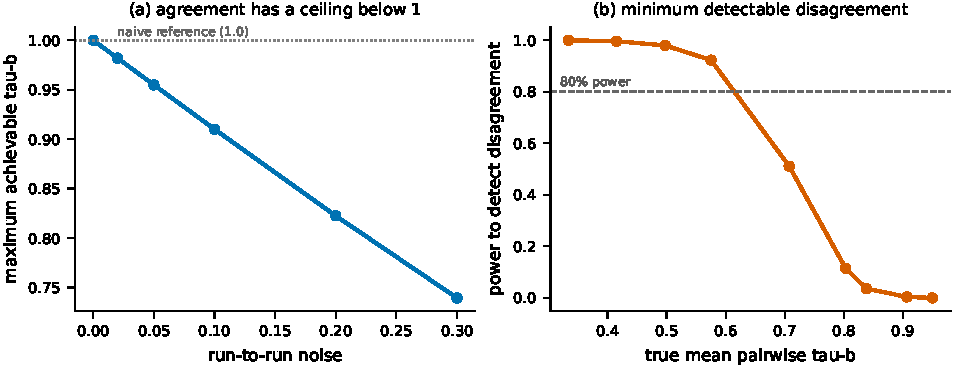
\includegraphics[width=0.85\textwidth]{F9_design_simulation.pdf}
\caption{Pre-specified design simulation: the agreement ceiling and the minimum detectable
disagreement.}
\label{fig:design}
\end{figure}

\section{Inventory of computations in the deposit}

Table~\ref{tab:release} accounts for every computation in the archive and
reconciles the ``4{,}400 run records'' quoted in the abstract with the
supplementary analyses added afterwards. Fit counts are recovered from the
deposited records rather than from design arithmetic.

\begin{table}[htbp]\centering\small
\caption{Every computation in the archive. The 4{,}400 figure quoted in the abstract is the
first block only; the rest are supplementary analyses, deposited alongside it. Fit counts
are recovered from the deposited records rather than from design arithmetic.}
\label{tab:release}
\footnotesize
\begin{tabular}{llr>{\raggedright\arraybackslash}p{0.27\textwidth}}
\toprule
Analysis & Design & Fits & Script \\
\midrule
\multicolumn{4}{l}{\textbf{Main designs -- the 4{,}400 run records}} \\
Arm~B, largest-first      & 100 cells $\times$ 16 pipelines       & 1{,}600 & \texttt{run\_arm\_b.py} \\
Arm~B, balance-preserving & 100 cells $\times$ 16 pipelines       & 1{,}600 & \texttt{run\_arm\_b.py} \\
Arm~A                     & 10 tasks $\times$ 24 $\times$ 5 seeds & 1{,}200 & \texttt{run\_arm\_a.py} \\
\cmidrule(lr){1-4}
\multicolumn{2}{l}{\emph{subtotal}} & \textbf{4{,}400} & \texttt{runs/all\_runs\_arm*.parquet} \\
\addlinespace
\multicolumn{4}{l}{\textbf{Supplementary analyses -- also deposited}} \\
Excluded-task runs        & 6 tasks $\times$ 24 $\times$ 5 seeds  & 720 & \texttt{run\_arm\_a\_excluded.py} \\
Equal tuning budget       & 5 rules $\times$ 16 $\times$ (6 + 1)  & 560 & \texttt{run\_equal\_tuning.py} \\
Depth $\times$ activation & 4 configs $\times$ 6 $\times$ 4 $\times$ 5 & 480 &
  \texttt{run\_depth\_\allowbreak activation\_\allowbreak ablation.py} \\
Negative-draw sensitivity & 5 rules $\times$ 5 draws $\times$ 12  & 300 & \texttt{run\_sensitivity\_draw.py} \\
Cluster-aware intervals   & 5 rules $\times$ 16; 5 tasks $\times$ 24 & 200 & \texttt{run\_cluster\_intervals.py} \\
SVM exact vs Nystr\"om    & 5 rules $\times$ 3 seeds $\times$ 2   &  30 & \texttt{check\_svm\_approximation.py} \\
Splitter stress test      & 15 cells $\times$ 4 splitters         &   0 & \texttt{run\_splitter\_stresstest.py} \\
Provenance overlap audit  & exact set intersection                &   0 & \texttt{tables/esm\_exposure\_*.csv} \\
Split definitions         & 200 Arm~B cells; 16 Arm~A datasets    &   0 & \texttt{export\_splits.py} \\
\cmidrule(lr){1-4}
\multicolumn{2}{l}{\emph{total model fits}} & \textbf{6{,}690} & \\
\bottomrule
\end{tabular}

\vspace{3pt}
\footnotesize\raggedright
The last three fit no models: the stress test performs 60 cluster assignments and 60
leakage searches over cached clusterings, the provenance audit is an exact set
intersection, and the split export regenerates partitions without fitting anything. The
cluster-interval analysis additionally performs $2 \times 2{,}000$ bootstrap resamples per
fit. \texttt{reproduce.sh} runs every stage above in order.

\paragraph{Split definitions.} \texttt{results/splits/} holds the exact partitions every
reported number was computed on: \texttt{armB\_splits.parquet} gives the test-row indices
for all 200 Arm~B cells (415{,}136 assignments across 5 rules $\times$ 4 thresholds
$\times$ 5 seeds $\times$ 2 splitters) against the canonical corpus ordering, whose SHA-256
fingerprint per rule is in \texttt{armB\_fingerprint.csv}; \texttt{armA\_splits.parquet}
gives all 52{,}316 released Arm~A rows with a per-sequence SHA-1, the split as published,
and whether we scored it. Sequences themselves are not redistributed, so a reader rebuilds
the corpus, checks the fingerprint, and -- if it matches -- has our partitions exactly. If
it does not match, that is visible immediately rather than after a silent comparison
against a different corpus.
\end{table}

\section{Negative-set construction, in full}
\label{sec:negaudit}

Each rule is a deterministic function of the positive set, the UniProt pool and a seed, and
is implemented in \texttt{bra/corpus.py} and \texttt{bra/negatives.py}. The positive set is
identical under all five rules: the published AMPBenchmark positives, non-standard residues
removed, length $\geq 5$, CD-HIT-reduced at 90\%, minus three homopolymers
(\texttt{PPPPPPPPPP}, \texttt{DDDDDDD}, \texttt{FFFFFFFF}) that are their own only
permutation and would otherwise be emitted as their own negatives under the shuffled rule.
Final positive set: 5{,}187 sequences.

The negative pool is reviewed UniProt (SwissProt), \textbf{retrieved 2026-10-05}: 575{,}749
records, of which 573{,}063 contain only the 20 standard residues. Duplicate \emph{sequences}
are removed before sampling, because SwissProt stores identical sequences under multiple
accessions and sampling rows without replacement can otherwise draw one sequence twice.
Class ratio is fixed at 1:1 for every rule, giving 10{,}374 sequences per corpus, and no
negative is byte-identical to any positive -- asserted at construction, not assumed.

\begin{table}[htbp]\centering\small
\caption{The five rules as implemented. Each draws against a per-rule \texttt{seen} set, so
no sequence appears twice within a corpus.}
\label{tab:negrules}
\begin{tabular}{llp{0.44\textwidth}}
\toprule
Rule & Source & Selection \\
\midrule
random UniProt      & SwissProt & uniform draw, length-filtered to 5--100 residues \\
annotation filtered & SwissProt & as above, excluding records keyworded
  \textit{Antimicrobial}, \textit{Antibiotic}, \textit{Fungicide} or \textit{Defensin} \\
length matched      & SwissProt & random contiguous fragments matching the positive
  length distribution \\
composition matched & SwissProt & fragments chosen from 60 candidates per positive,
  minimising $L_1$ distance in amino-acid composition \\
shuffled positives  & positives & each positive randomly permuted \\
\bottomrule
\end{tabular}
\end{table}

\paragraph{Annotation filtering does not guarantee a clean negative class, and we do not
claim it does.} The filter removes records carrying four UniProt keywords. It cannot remove
an antimicrobial peptide that has never been annotated as one, and most of SwissProt has
not been assayed for antimicrobial activity. The negative class under that rule is better
described as \emph{not known to be antimicrobial} than as \emph{not antimicrobial}, and
some unknown fraction of it is mislabelled. That bounds how well any model can legitimately
score under the rule, and means a model penalised for calling such a sequence positive may
be right. It also makes the annotation-filtered and random-UniProt rules more similar than
their names suggest, which the results bear out: they agree closely on difficulty, on
provenance (Table~\ref{tab:exposure}) and on residual leakage (Table~\ref{tab:leakcell}).
We report them as two rules because the literature treats them as two, not because we can
show the filter works.

Accessions are not redistributed: the positives derive from DBAASP through AMPBenchmark and
the negatives from UniProt, and those terms govern redistribution. The construction scripts
are released with SHA-256 hashes of both inputs, and \texttt{reproduce.sh} fails on a hash
mismatch rather than proceeding with different negatives.

\section{What the leakage audit measures}
\label{sec:leakdef}

Two distinct quantities are reported in the paper and should not be conflated.

\textbf{Exact duplicates} are byte-identical sequences in both partitions. They are found by
string comparison, are fatal regardless of any threshold, and in Arm~B are excluded by
construction and asserted per cell. In the Arm~A collection they are \emph{measured}, not
prevented: 336 across all 16 datasets, 315 in the ten used (Table~\ref{tab:armacounts}).

\textbf{Residual pairwise similarity} is a different quantity, and is what the $21.6\%$
figure refers to. For each cell we run an explicit MMseqs2 search of the test partition
against the training partition at the cell's own identity threshold and coverage $0.8$, and
report
\[
\text{leak fraction} \;=\;
\frac{\#\{\text{test sequences with} \geq 1 \text{ training hit at or above the threshold}\}}
     {\#\{\text{test sequences}\}} .
\]
It is a fraction of \emph{test sequences}, not of pairs, so one test sequence with fifty
training neighbours counts once. The $21.6\%$ is the mean over the five rules at the 40\%
threshold under the pre-registered splitter; it is not pooled across thresholds.

\begin{table}[htbp]\centering\small
\caption{Residual leakage per cell, mean over five seeds, pre-registered splitter. The
\texttt{random} column is an unclustered control and is exactly zero because no clustering
is performed. Leakage rises as the nominal threshold \emph{tightens}, in every rule.}
\label{tab:leakcell}
\begin{tabular}{lrrrr}
\toprule
Negative rule & 90\% & 70\% & 40\% & random \\
\midrule
random UniProt      & 0.0167 & 0.1687 & \textbf{0.3925} & 0.000 \\
annotation filtered & 0.0175 & 0.1842 & \textbf{0.3811} & 0.000 \\
composition matched & 0.0126 & 0.0429 & 0.1098 & 0.000 \\
length matched      & 0.0122 & 0.0461 & 0.1016 & 0.000 \\
shuffled positives  & 0.0113 & 0.0429 & 0.0965 & 0.000 \\
\midrule
pooled mean         & 0.0141 & 0.0970 & \textbf{0.2163} & 0.000 \\
\bottomrule
\end{tabular}
\end{table}

\paragraph{Why tightening the threshold increases residual leakage.} This reads as a
paradox and is not one. The threshold does two things at once. It defines which pairs
\emph{count} as leakage, and it defines how sequences are grouped into clusters. Lowering it
to 40\% makes the counting criterion far more permissive -- short peptides clear 40\%
identity against unrelated sequences routinely -- so many more pairs qualify. It also
produces fewer, larger clusters, and because greedy clustering assigns each sequence to its
nearest representative rather than forming equivalence classes, two sequences can exceed
40\% identity with each other while sitting in different clusters. The second effect is why
cluster-disjointness fails to imply pairwise-disjointness; the first is why the failure is
large. Both grow as the threshold falls, and they compound. The effect is strongest for
whole-protein negatives (39\%), which are long enough to accumulate chance local
similarity, and weakest for shuffled positives (10\%), because a permutation destroys the
alignable order MMseqs2 searches on.

\section{Class balance, and what it does to each metric}
\label{sec:balmetric}

The class-balance failure is not a footnote to the splitting method; it is the mechanism by
which that method corrupts scores. Per-cell achieved balance under both splitters is in
Table~\ref{tab:balanceaudit}. Here we quantify what it does to the reported number.

Across the 100 pre-registered cells, correlating each cell's mean score with its test
positive fraction:

\begin{center}\small
\begin{tabular}{lrlr}
\toprule
Metric & $r$ & Metric & $r$ \\
\midrule
MCC               & $\mathbf{-0.887}$ & accuracy & $-0.530$ \\
balanced accuracy & $-0.712$          & AUPRC    & $+0.416$ \\
AUROC             & $-0.703$          & F1       & $-0.188$ \\
\bottomrule
\end{tabular}
\end{center}

\noindent MCC -- the paper's primary metric -- is the \emph{most} sensitive of the six.
AUPRC moves in the opposite direction, as expected for a measure that rewards a prevalent
positive class, and F1 is nearly inert. A benchmark reporting a single metric on an
unbalanced cluster-disjoint split is therefore reporting a number substantially set by a
partitioning side-effect, and its choice of metric determines both the magnitude and the
sign of that contamination.

This is also why the variance decomposition differs between the two grids: under
largest-first assignment the threshold drives class balance, class balance drives MCC, and
the threshold consequently absorbs $14.9\%$ of score variance that is not about partition
difficulty at all. Under the balance-preserving splitter the same component is $0.6\%$.

\section{The variance-component model}
\label{sec:varmodel}

\textbf{Model.} A fully crossed random-effects design on pipeline, negative rule, clustering
threshold and seed, with one observation per cell. The Arm~B grid is a complete balanced
factorial ($16 \times 5 \times 4 \times 5 = 1{,}600$ cells per metric), so the orthogonal
decomposition is exact and the expected-mean-square equations solve in closed form,
top-down from the four-way interaction, which absorbs the residual. For a factor subset $A$,
\[
\mathbb{E}[\mathrm{MS}_A] \;=\;
\sum_{C \supseteq A} \Big( N \big/ \textstyle\prod_{f \in C} n_f \Big)\, \sigma^2_C .
\]

\textbf{Assumptions.} Effects additive on the MCC scale and exchangeable within each factor;
residuals homoscedastic across cells. Balance is required and holds by construction. The
point estimates are moment estimators and need no normality assumption; the jackknife
intervals assume only that seeds are exchangeable replicates.

\textbf{Uncertainty.} Delete-one-seed jackknife, which preserves the balance the
decomposition requires. Resampling cells destroys it, and when we tried that it produced
intervals excluding their own point estimates. Intervals for both grids are in the main
text.

\textbf{Population.} The estimate applies to \emph{this corpus, these five rules, these four
thresholds and these sixteen pipelines}. A variance share is a property of a design, not of
a field: widening the pipeline set or narrowing the rule set would move every number in the
table. We make no claim that $71\%$ is a universal property of peptide prediction. What
travels is the \emph{ordering} of components, which is identical under both splitters.

\textbf{Negative estimates.} Two components (seed, and pipeline $\times$ rule $\times$ seed)
return small negative variances of order $-10^{-6}$, the expected behaviour of a moment
estimator at a true zero. They are reported unclipped in
\texttt{armB\_mom\_variance\_components.csv} and clipped only when converting to
percentages, because silently clipping is how a structural zero becomes a precise
measurement.

\section{Sensitivity to the task-inclusion cutoff}
\label{sec:cutoff}

Arm~A uses the ten tasks with at least 900 training sequences. Justifying an exclusion is
weaker than showing what including the excluded data does, so we ran the six omitted
datasets through the identical zoo, seeds and procedure -- a further 720 fits, no failures,
written to a separate directory so the reported ten-task result could not be contaminated
(\texttt{run\_arm\_a\_excluded.py}). The cutoff can then be moved in both directions.

\begin{table}[htbp]\centering\small
\caption{Arm A rank agreement under alternative training-size cutoffs, with all sixteen
released datasets available. Agreement falls as smaller tasks are added and rises as they
are removed; the reported cutoff is the conservative choice, not a favourable one.}
\label{tab:cutoff}
\begin{tabular}{lrrrr}
\toprule
Cutoff ($n_\text{train}$) & tasks & $\tau_b$ & ceiling & normalised \\
\midrule
all 16 datasets                & 16 & 0.292 & 0.778 & \textbf{0.375} \\
$\geq 200$                     & 15 & 0.309 & 0.789 & 0.391 \\
$\geq 350$                     & 12 & 0.379 & 0.812 & 0.467 \\
$\geq 700$                     & 10 & 0.479 & 0.838 & 0.572 \\
$\geq 900$ \textbf{(reported)} & 10 & 0.479 & 0.838 & \textbf{0.572} \\
$\geq 1{,}300$                 &  8 & 0.501 & 0.850 & 0.589 \\
$\geq 1{,}600$                 &  6 & 0.573 & 0.872 & 0.657 \\
$\geq 3{,}000$                 &  5 & 0.564 & 0.879 & 0.641 \\
\bottomrule
\end{tabular}
\end{table}

\textbf{Including the excluded datasets strengthens the finding rather than weakening it.}
Across all sixteen, normalised agreement is $0.375$ against the $0.572$ we report: rankings
transfer \emph{worse} once the small tasks are admitted. Part of that is genuine -- more
tasks, more biological heterogeneity -- and part is that tiny test sets rank noisily, which
is why the seed ceiling falls too, from $0.838$ to $0.778$. The normalised statistic already
divides by that ceiling, so the comparison is not merely a noise artefact. In the other
direction, restricting to the five largest tasks lifts normalised agreement only to
$0.641$, still far below the pre-specified threshold of $0.85$.

The conclusion is therefore insensitive to the cutoff across the whole range the data
permit, $0.375$ to $0.657$, and the value we report sits in the middle rather than at the
flattering end. Two further details. The cutoff falls in a real gap in the size
distribution -- no dataset has between 698 and 948 training sequences, so the $\geq 700$ and
$\geq 900$ rows are identical and the threshold is not tuned to a boundary. And the six
omitted datasets (antioxidant 698, anti-parasitic 482, quorum sensing 349, anti-MRSA 237,
anti-MAP 221, blood--brain barrier 191) were excluded on size alone, before any pipeline was
fitted; their sizes and duplicate counts are in Table~\ref{tab:armacounts}.

\section{Architecture sensitivity: MLP depth and activation}
\label{sec:ablation}

The main grid fixes the MLP learner at one hidden layer of 256 units with ReLU, frozen
before corpus construction so that protocol preference could not be confounded with search
effort. This section asks what that choice cost, as a \textbf{supplementary sensitivity
analysis that does not revise the main results and is not merged into them}.

Depths $1, 3, 4, 5, 6, 7$ were crossed with four activations and five seeds on three Arm~A
tasks, plus a capacity-controlled repeat of one task under a pyramid width policy:
$4 \times 120 = \mathbf{480}$ fits, all of which converged. The representation is
mean-pooled ESM-2 35M throughout, and every other setting is held at the value the main
grid used. The \texttt{identity} activation is not padding: a stack of identity-activated
layers collapses to a single linear map whatever its depth, so its distance from the best
non-linear row measures how much non-linearity the task needed at all.

\begin{table}[htbp]\centering\small
\caption{Depth effect against the seed noise floor, per configuration. The floor is the
median within-cell standard deviation of MCC across five seeds; a depth effect smaller than
roughly twice it is not a depth effect. \emph{Identity gap} is the distance from the best
non-linear activation to the linear control, in units of that floor.}
\label{tab:ablsummary}
\begin{tabular}{lrrrlrl}
\toprule
Task & floor & spread & ratio & best cell & id.\ gap & reading \\
\midrule
AMP            & 0.0156 & 0.0108 & 0.69 & d7 ReLU              & 4.3$\times$ & depth null \\
AMP (pyramid)  & 0.0135 & 0.0124 & 0.92 & d4 ReLU              & 4.9$\times$ & depth null \\
toxicity       & 0.0286 & 0.0441 & 1.54 & \textbf{d1} tanh     & 0.9$\times$ & depth hurts \\
antibacterial  & 0.0134 & 0.0258 & 1.92 & \textbf{d1} logistic & 1.1$\times$ & depth hurts \\
\bottomrule
\end{tabular}
\end{table}

\begin{table}[htbp]\centering\small
\caption{Mean MCC by depth, averaged over the four activations and five seeds. Depth~1 is
the published configuration. No column improves materially with depth, and two decline.}
\label{tab:abldepth}
\begin{tabular}{lrrrr}
\toprule
Depth & AMP & AMP (pyramid) & toxicity & antibacterial \\
\midrule
\textbf{1} (published) & 0.3099 & 0.3099 & \textbf{0.3565} & \textbf{0.4471} \\
3 & 0.3006 & 0.3120 & 0.3446 & 0.4217 \\
4 & 0.3114 & 0.3076 & 0.3389 & 0.4213 \\
5 & 0.3060 & 0.3044 & 0.3302 & 0.4295 \\
6 & 0.3047 & 0.3047 & 0.3295 & 0.4301 \\
7 & 0.3104 & 0.2996 & 0.3124 & 0.4220 \\
\bottomrule
\end{tabular}
\end{table}

\paragraph{Depth buys nothing, and sometimes costs.} On AMP the spread across six depths is
smaller than the spread across five reseedings of a single depth (ratio $0.69$), and the
capacity-controlled pyramid repeat agrees ($0.92$), so the null is not an artefact of
confounding depth with parameter count. On toxicity and antibacterial the ratio rises to
$1.54$ and $1.92$ -- still under the conventional factor of two, but the sign is consistent
and the direction is downward: on both, \textbf{the published single-layer configuration is
the best cell outright}, and depth~7 costs $0.044$ MCC on toxicity relative to depth~1. The
published configuration is therefore retained on parsimony: $123{,}650$ parameters against
$518{,}402$ at depth~7, with no detectable gain anywhere and a loss on two tasks of three.

\paragraph{How much non-linearity each task needs does not transfer.} On AMP the linear
control sits $4.3$ noise floors below the best non-linear activation: that task genuinely
needs a non-linear decision surface, and one hidden layer supplies it. On toxicity and
antibacterial the same gap is $0.9$ and $1.1$ floors -- within noise, meaning those two
tasks are close to \emph{linearly separable} in ESM-2 35M space. The ordering of
activations differs too: ReLU leads on AMP and toxicity, logistic on antibacterial, where
the linear control also edges out ReLU ($0.4232$ against $0.4202$). An architectural
recommendation read off any one of these three tasks would mislead on the other two --
the same conclusion Arm~A reaches for pipelines, reached here independently.

\paragraph{Where the errors go.} Summed over five seeds on AMP ($12{,}830$ predictions),
moving from the published configuration to its nominal best cell trades $207$ false
negatives for $124$ false positives: sensitivity $0.5573 \to 0.5895$, specificity
$0.7639 \to 0.7445$, a net $83$ fewer errors. The direction suits screening, where a missed
active costs more than a false lead, but the magnitude is inside what reseeding moves and
no decision should rest on it. The linear control is the most conservative of the three
(specificity $0.7900$) and pays for it in the failure mode that matters, missing $3{,}581$
of $6{,}410$ actives.

\paragraph{Limitations.} One representation (ESM-2 35M) and three of ten tasks. Learning
rate, dropout and patience were held fixed across depths, and deeper networks are more
sensitive to all three, so a per-depth tuned sweep would answer a different question than
this one -- whether depth helps \emph{at the paper's own settings}. Constant width
confounds depth with capacity; the pyramid policy separates them and agrees. One
optimisation outlier is reported rather than dropped: depth~6 with identity activation at
seed~0 on AMP required \SI{2645}{\second} against a \SI{9}{\second} median for its depth,
converged, and scored in line with its neighbours. Per-run records, confusion matrices for
all 480 cells and the generated summaries are in \texttt{results/ablation\_depth/}.

\end{document}
